\documentclass[11pt]{article}
\usepackage{fancyhdr}
\usepackage[letterpaper, margin=1in]{geometry}
%\usepackage{indentfirst}
\usepackage{graphicx}
\usepackage{amsmath}
\usepackage{amssymb}
\usepackage{siunitx}
\sisetup{detect-weight=true, detect-family=true} % makes siunitx follow font formatting like bold, italic, etc.
\usepackage{cancel}
\usepackage{isotope}
\usepackage{listings}
\usepackage[dvipsnames,table]{xcolor}
\usepackage{xspace}
\usepackage{booktabs} % makes tables pretty
\usepackage{longtable} % for long tables
\usepackage{multirow} % makes tables pretty
\usepackage{multicol} % makes tables pretty
\usepackage{setspace}
\usepackage{subcaption}
\usepackage[font={bf}]{caption}
\usepackage[utf8]{inputenc}
\usepackage{textcomp}
\usepackage{titlesec}
\usepackage{svg}
\usepackage{pdflscape} % makes pages landscape
\usepackage{mathtools}
\usepackage{enumitem}
\usepackage[T1]{fontenc}
\usepackage{tikz}
\usepackage{soul}

\usepackage{hyperref}
\usepackage{cleveref}
\newcommand{\creflastconjunction}{, and\nobreakspace} % adds oxford comma to cleveref

\doublespacing

% bib if needed
\bibliographystyle{ieeetr}


% fancy header stuff
\usepackage{fancyhdr}
\pagestyle{fancy}

\setlength{\headheight}{28pt}
\lhead{ME 568 / OC 674\\Spring 2022}
\chead{Assignment 5\\}
\rhead{Austin Warren\\Due June 6, 2022}

\begin{document}

\begin{enumerate}

    % part 1
    \item \textbf{Part 1: Scales of Turbulence} Estimate characteristic velocity and length scales of the turbulence. Can you use these scales to determine the dissipation rate? What is the Taylor microscale? Kolmogorov lengthscale? Does the model actually resolve the smallest turbulent scales? How do each of these scales vary with time? Is their variability consistent with your expectations? Can you also estimate a timescale for largest scale motions? And the smallest scale motions? Briefly explain how/whether/why these are consistent with your expectations.\par
    
%    Ideas:
%    \begin{itemize}
%        \item correlation to find length scale -- or just use physical limits of problem $\ell = \int_0^{\infty}\rho(x)dx$
%        \item not sure on characteristic velocity scale -- just square root tke, lol
%        \item $\frac{u^3}{\ell}$ for dissipation once I know the velocity and length
%        \item Kolmogorov scale is where Re=1; also $\eta=\left( \epsilon/\nu \right)^{1/2}$; $\eta=\left(\nu^3/\epsilon\right)\sim L Re^{-3/4}$
%        \item Taylor microscale relates characteristic velocity and dissipation $\frac{\lambda}{L} \sim Re_L^{-1/2}$ and $\epsilon = 15\nu u^2 / \lambda^2$ for isotropic turbulence -- Liburdy says to use correlation thing for Taylor microscale $1+\frac{r^2}{2}\frac{\partial^2\rho}{\partial r^2} = 1-\frac{r^2}{\lambda^2}$
%        \item compare characteristic time scale to time scale determined with frozen turbulence ($\ell/U$ and $L/U$); also $\frac{tke}{\epsilon}=\frac{u^2}{u^3/\ell}=\frac{u}{\ell}$
%    \end{itemize}
	To get the characteristic velocity, I added up the total tke at each time step, then took the square root of the tke. This may result in a larger than is realistic velocity, but it is a good measure of the energy contained in the turbulence. For the characteristic length scale, I used the integral length scale calculated from integrating the auto-correlation function over the length of the problem. I selected $u^{\prime}$ to use for the auto-correlation. I used a correlation function provided by another student, which seems to work well. I performed the correlation at each $z$ slice of the problem at each time step, then selected the largest value for each time step to get the length scale. Similarly to the characteristic velocity, this may not be entirely realistic, but it will represent the largest scales for the turbulence.
	\begin{equation}
		\ell = \int\limits_0^{\infty} \rho (r) dr
	\end{equation}
	For the Taylor microscale, I used the Taylor expansion estimate from the correlation function. I calculated the correlation function at each $z$ slice, then took the median of all $z$ slices for each time step. I felt that this was a better representation of the length scale than the maximum or minimum and averaging with a mean may have skewed results since some of the individually calculated values can be extreme at each point.
	\begin{equation}
		1+\frac{r^2}{2}\frac{\partial^2\rho}{\partial r^2} = 1-\frac{r^2}{\lambda^2}
	\end{equation}
	Finally for the Kolmogorov length scale, I assumed that the Reynolds number will be one at this scale and used velocity and viscosity to solve for the length scale. I was not sure what velocity to use, but I thought the fluctuating velocity, $u^{\prime}$, would be a good representation of the velocity at that scale. I calculated this at each point, then averaged over each $z$ slice, then used the median of the $z$ slices for each time step like for the Taylor microscale. I also calculated the Kolmogorov length scale using the viscosity and dissipation. I do not believe my dissipation values are correct because I am leaving out changes in the $y$ direction, which will reduce the total dissipation calculated, but I thought it would be good to compare trends with the Reynolds number method.
	\begin{equation}
		Re = 1 = \frac{u^{\prime} \eta}{\nu}
	\end{equation}
	\begin{equation}
		\eta = \left( \nu^3 / \epsilon \right)^{1/4}
	\end{equation}
	\Cref{fig:length} shows the characteristic length scale ($\ell$), the Taylor microscale ($\lambda$), and the Kolmogorov length scale ($\eta$) over time.
	\begin{figure}[htbp]
		\centering
		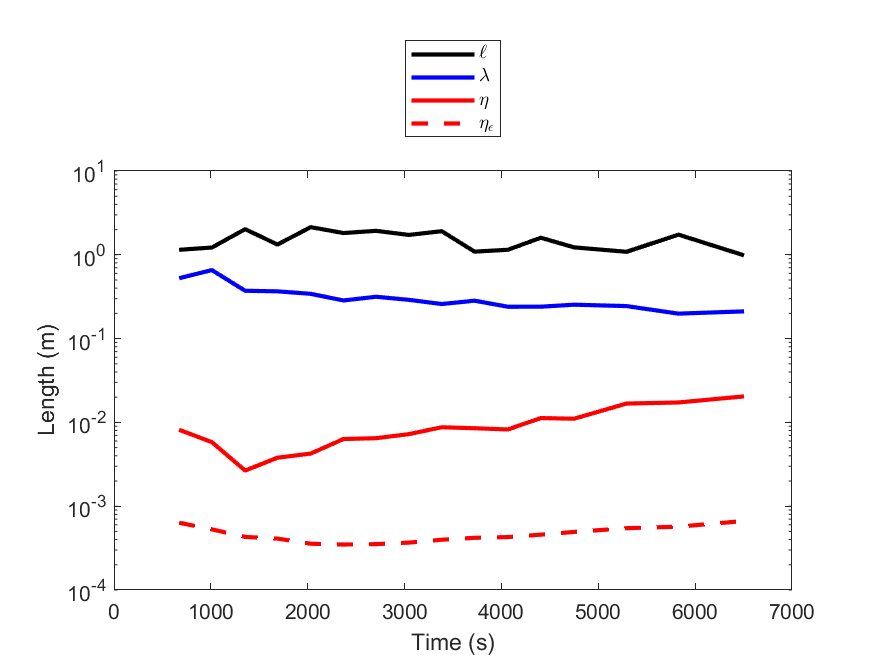
\includegraphics[width=\textwidth]{1-plots/char_length_comp_plot.png}
		\caption{The characteristic length scale ($\ell$), the Taylor microscale ($\lambda$), and the Kolmogorov length scale ($\eta$) over time.}
		\label{fig:length}
	\end{figure}
    The characteristic length scale stays about constant over the evolution of the flow and is approximately equal to the physical constraint in the $z$ direction, which is a good sign since the turbulence cannot be larger than the physical confines of the problem. The Kolmogorov length scale is only 2-3 orders of magnitude lower than the characteristic length scale, which is not as much gap as I was expecting, but it could be explained by my use of the fluctuating velocity for the Reynolds number. More importantly, the Kolmogorov length scale increases over time, which is what we expect for a turbulent system with no added source of turbulence. As the tke dissipates away, the smallest length scales get larger while the largest length scales remain the same. This plot shows both of these trends. The Taylor microscale is larger than I was expecting, but still falls between the other two scales. It decreases over time, which is not what I was expecting visually when I first saw it, but I believe it is the correct behavior. Since the ratio of the Kolmogorov and Taylor lengths scales with the Reynolds number to a fraction, as the Reynolds number decreases, the difference between the two lengths decreases less and the gap between them would close.
    
    I calculated the characteristic velocity by taking the square root of the tke, as said above. To calculate the velocity at the small scales, I used the Kolmogorov velocity calculated with viscosity and dissipation. \Cref{fig:vel plot} shows both velocity scales plotted over time.
    \begin{equation}
    	u_{char} = \sqrt{tke}
    \end{equation}
	\begin{equation}
		u_{\eta} = \left( \nu\epsilon \right)^{1/4}
	\end{equation}
    \begin{figure}[htbp]
    	\centering
    	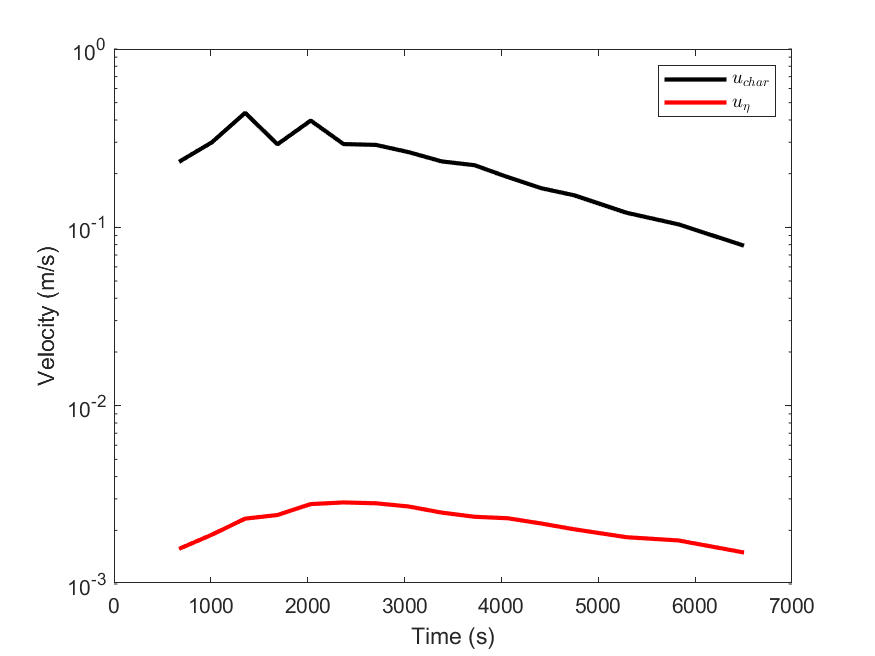
\includegraphics[width=\textwidth]{1-plots/char_vel_plot.png}
    	\caption{Characteristic and Kolmogorov velocity scales.}
    	\label{fig:vel plot}
    \end{figure}
	The two velocity scales are a similar order of magnitude apart as their length scale counterparts and they follow a similar trend. As the total energy in the system is dissipated, the velocity will decrease, so the trend downwards after the initial increase from production is what we expect.
	
	For the large scale time, I used the calculated characteristic length and velocity scales. To get a small time scale, I used the Kolmogorov time scale calculated with the viscosity and dissipation rate. \Cref{fig:time plot} shows both scales over time.
	\begin{equation}
		t = \frac{\ell}{u}
	\end{equation}
	\begin{equation}
		\tau_{\eta} = \left( \nu/\epsilon \right)^{1/2}
	\end{equation}
    \begin{figure}[htbp]
    	\centering
    	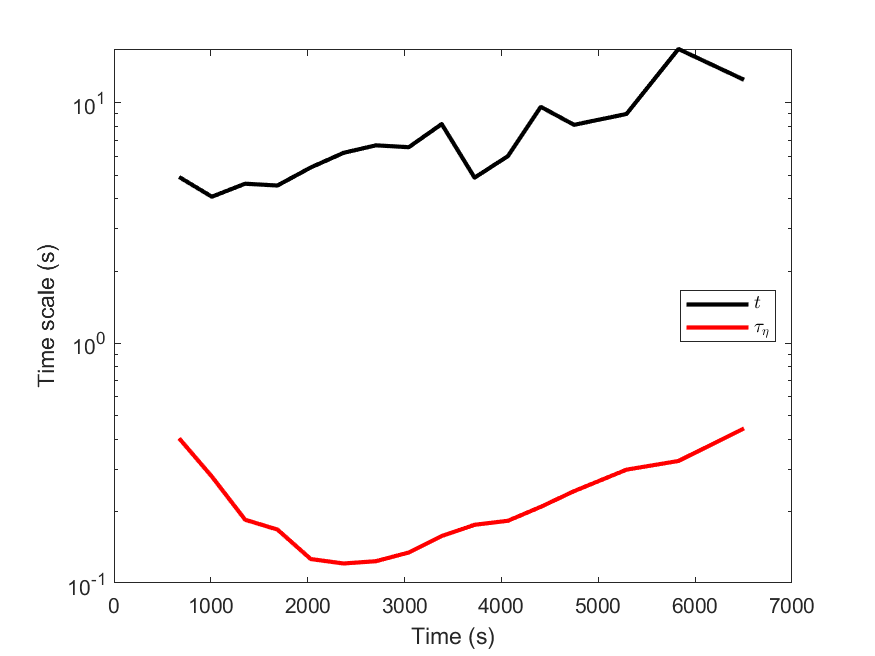
\includegraphics[width=\textwidth]{1-plots/char_time_plot.png}
    	\caption{Large and small time scales over time.}
    	\label{fig:time plot}
    \end{figure}
	Both scales trend in the same direction after the small scale time dips down from the initial production. As energy is dissipated, it makes sense that the time scales would increase and things would take longer to move around. The gap between the time scales is not very large compared to the length or velocity scales, but since the velocity and length scales are similar orders of magnitude apart, it is expected that the time scales are similar in order of magnitude.




    
	\clearpage
    % part 2
    \item \textbf{Part 2: Eddy Viscosity} There are several ways that one can estimate an eddy viscosity. From the data, determine an ``eddy viscosity'' for this flow. Does your estimate evolve in time, and if so, how does it vary? Can you determine some average value for it? And then, is there a way in which you can determine/verify whether your estimate is approximately correct?
    
%    Ideas:
%    \begin{itemize}
%        \item $\overline{u_i u_j} = \nu_T \frac{\partial u_i}{\partial x_j}$
%        \item $\nu_T = \left( tke \right)^{1/2} \ell$ -- this is what Liburdy said in class
%        \item $\nu_T \left( \frac{\partial U}{\partial z} \right)^{2} = \epsilon$
%        \item $\frac{\partial U}{\partial t} = \nu_T\frac{\partial^2 U}{\partial z^2}$ -- plugging back into momentum equation to check
%    \end{itemize}

	\Cref{fig:nuT} shows the estimate of eddy viscosity using the tke and characteristic length in the form:
	\begin{equation}
		\nu_T = \left( tke \right)^{1/2} \ell = u \ell\:.
	\end{equation}

	\begin{figure}[htbp]
		\centering
		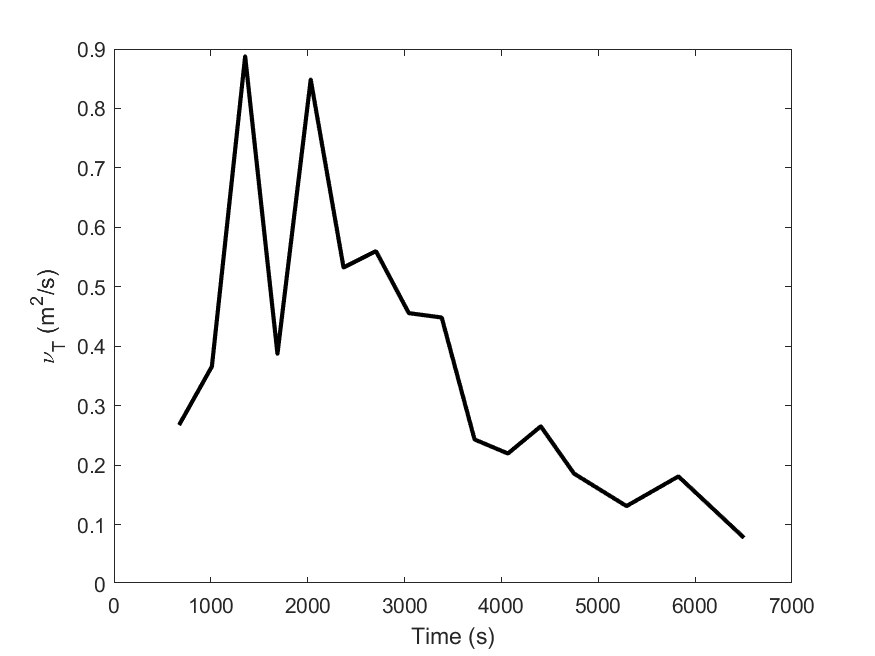
\includegraphics[width=\textwidth]{1-plots/char_nuT_plot.png}
		\caption{Eddy viscosity estimate over time using characteristic length and velocity.}
		\label{fig:nuT}
	\end{figure}
    
	\clearpage
    % part 3
    \item \textbf{Part 3: Turbulent Spectra} Compute the turbulent energy spectrum that characterizes one component of the velocity fluctuations at a given timestep (it is usually useful to average a number of spectra together in a quasi-homogeneous region to reduce noise/uncertainty). Does the spectrum look like you would expect it to? Do this for all the timesteps and plot on a single plot. Do the spectra vary in a way that is consistent with your expectations? Can you estimate the dissipation rate from those spectra, and is it consistent with your previous estimates?
    
%    Ideas:
%    \begin{itemize}
%        \item Dr. Nash said something about giving us a matlab file to calculate spectra?
%    \end{itemize}


	I used Dr. Nash's provided power spectral density function. I averaged over the first ten $z$ slices at each time step, since the bottom of the problem looks mostly homogeneous at each time. \Cref{fig:psd} shows the power spectral density for each time step. I am not sure what the units of the frequency are, but I believe I should be able to relate frequency to something else and get a wave number. The sprectra start out very nice looking with a clear -5/3 looking region (I have not checked to see if this is actually the slope yet), but as time goes on, the spectra get more messy. If the $x$-axis of the plot was wave number, $k$, I would expect the curves to move toward smaller wave numbers over time as well as losing the linear section. 

	\begin{figure}[htbp]
		\centering
		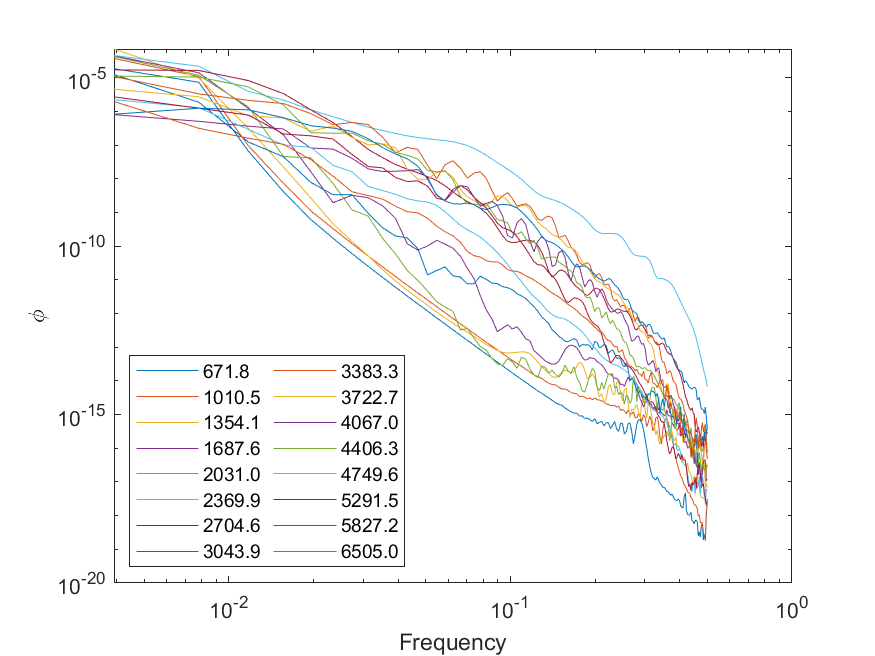
\includegraphics[width=\textwidth]{1-plots/psd_plot.png}
		\caption{Power spectral density for all time steps.}
		\label{fig:psd}
	\end{figure}



\end{enumerate}








\end{document}